% !TEX program = xelatex
% !TEX root = main.tex
\documentclass[12pt, a4paper]{article}

% --- PACOTES ---
% Essenciais e de Idioma
\usepackage[brazilian]{babel}
\usepackage{fontspec}

% Layout e Geometria
\usepackage[margin=2.5cm]{geometry}
\usepackage{fancyhdr}
\usepackage{titlesec}
\usepackage{titling}
\usepackage{authblk}

% Matemática e Física
\usepackage{amsmath,amssymb,amsfonts,mathtools,amsthm}
\usepackage{physics}               % Comandos como \dd, \grad, \vb, etc.
\usepackage{tensor}                % Para tensores com índices
\usepackage{bm}                    % Símbolos matemáticos em negrito
\usepackage{cancel}                % Para cortar expressões matemáticas

% Referências e Links
\usepackage{hyperref}
\usepackage{cleveref}              % Referências inteligentes (\cref{...})
\usepackage{bookmark}              % Melhora os bookmarks do PDF

% Bibliografia e Citações
\usepackage{csquotes}              % Necessário para alguns estilos do biblatex
\usepackage[backend=biber, style=numeric-comp, sorting=none]{biblatex}


% Visual
\usepackage{graphicx}
\usepackage{xcolor}
\usepackage{enumitem}              % Controle avançado de listas
\usepackage{footnote}
\usepackage{manyfoot}              % Múltiplos tipos de notas de rodapé
\usepackage{tocloft}               % Para customizar o sumário
\usepackage{lipsum}                % Apenas para texto de exemplo
\usepackage{comment}               % Serve pra comentar blocos inteiros



% --- AMBIENTES ---
\newtheoremstyle{meuremarkstyle} % <name>
  {\topsep}                   % <space above>
  {\topsep}                   % <space below>
  {\normalfont}               % <body font> - texto normal para o conteúdo
  {}                          % <indent amount>
  {\itshape}                 % <head font> - italico para o título
  {:}                         % <head punctuation> - AQUI ESTÁ O SEGREDO: dois pontos!
  {.5em}                      % <space after head>
  {\underline{\thmname{#1}}}  % <head spec> - deixar vazio para o padrão
\theoremstyle{meuremarkstyle}
\newtheorem*{notação}{Notação}

\newtheoremstyle{definicao} % <name>
  {\topsep}                   % <space above>
  {\topsep}                   % <space below>
  {\normalfont}               % <body font> - texto normal para o conteúdo
  {}                          % <indent amount>
  {\itshape}                 % <head font> - italico para o título
  {:}                         % <head punctuation> - AQUI ESTÁ O SEGREDO: dois pontos!
  {.5em}                      % <space after head>
  {\underline{\thmname{#1}}}  % <head spec> - deixar vazio para o padrão
\theoremstyle{definicao}
\newtheorem*{definição}{Definição}



% --- CONFIGURAÇÃO DA BIBLIOGRAFIA ---
\addbibresource{referencias.bib}

% --- CONFIGURAÇÕES VISUAIS ---
% Parágrafos (sem indentação, com espaçamento)
\setlength{\parskip}{0.5em}
\setlength{\parindent}{0pt}

% Fonte Principal
\setmainfont{Latin Modern Roman} % Fonte padrão moderna, segura e completa

% Cabeçalho e Rodapé (Fancyhdr)
\pagestyle{fancy}
\fancyhf{} % Limpa todos os campos do cabeçalho e rodapé
\fancyhead[L]{\nouppercase{\leftmark}} % Esquerda: Seção atual (sem caixa alta)
\fancyhead[R]{\thepage}                 % Direita: Número da página
\renewcommand{\headrulewidth}{0.4pt}
\renewcommand{\sectionmark}[1]{\markboth{#1}{}}


% Formato dos Títulos (Titlesec)
\titleformat{\section}{\large\bfseries}{\thesection.}{1em}{}
\titleformat{\subsection}{\normalsize\bfseries}{\thesubsection}{1em}{}
\titleformat{name=\section, numberless}
  {\large\bfseries\centering}
  {}
  {0pt}
  {}

% Sumário Pontilhado (Tocloft)
\renewcommand{\cftsecleader}{\cftdotfill{\cftdotsep}}

% Notas de Rodapé (Manyfoot)
\DeclareNewFootnote{B}[fnsymbol]

% Configurações de Links (Hyperref)
\hypersetup{
    colorlinks=false,
    linkcolor=blue,
    citecolor=red,
    urlcolor=magenta,
    pdftitle={Título do Trabalho Final},
    pdfauthor={Primeiro Autor; Segundo Autor}, % Autores no metadata do PDF
}

% %%%%%%%%%%%%%%%%%%%%%%%%%%%%%%%%%%%%%%%%%%%%%%%%%%%%%%%
%                         DOCUMENTO
% %%%%%%%%%%%%%%%%%%%%%%%%%%%%%%%%%%%%%%%%%%%%%%%%%%%%%%%

\begin{document}
\pagenumbering{gobble}
% --- PÁGINA 1: TÍTULO, AUTOR E SUMÁRIO ---
\title{Diagramas de Carter-Penrose no Estudo de Buracos Negros}


\author{João Paulo Monteiro\\ Felipe Khalil}

\date{\today}

\maketitle
\tableofcontents

\newpage % Inicia o conteúdo na próxima página

% --- SEÇÕES DO TRABALHO (A partir da Página 1) ---
\pagenumbering{arabic}
\setcounter{page}{1}
\section{Introdução}

Uma das primeiras dificuldades que surgem em relatividade geral no estudo de buracos negros
 é a falta de uma representação visual e geométrica do que está acontencendo no entorno
desses objetos. Tais representações não são, de fato, \textit{necessárias} para o 
entendimento da física de buracos negros; contudo, veremos que serão de grande utilidade para explicitar
(e até revelar) algumas propriedades fundamentais do espaço-tempo na presença de corpos massivos.

Mas para quê mais diagramas? - alguém pode se perguntar. Afinal, o diagrama de Minkowisky cumpre bem sua função para um espaço-tempo plano, vazio de matéria e homogêneo; a princípio,
bastaria buscar algum tipo de \enquote{extensão natural} desse diagrama para espaços-tempos curvos, mantendo a estrutura cartesiana.
É isso que iremos fazer agora, e pelo título do nosso trabalho, já adiantamos que coisas
não muito agradáveis surgirão dessa primeira alternativa.

\subsection{Diagrama de espaço-tempo nas coordenadas de Schwartzschild}
Considere a métrica de Schwartzchild, a única solução com simetria esférica da
equação de Einsten no vácuo, expressa em coordenadas esféricas $(t,r,\theta,\varphi)$:
\begin{equation*}
  g = -\qty(1-\frac{2GM}{r})dt\otimes dt + \qty(1-\frac{2GM}{r})^{-1}dr\otimes dr + r^2\qty(d\theta \otimes d\theta + \sin^2\theta d\varphi \otimes d\varphi)
\end{equation*}

\begin{notação}
sempre que tivermos dois produtos tensoriais envolvendo coordenadas idênticas, escreveremos de forma mais
\enquote{relaxada}; e mesmo se não forem idênticas, ainda omitiremos o símbolo de produto tensorial, apenas tomando o cuidado de
respeitar a ordem dos produtos, como segue:
\begin{gather*}
  dx^{\mu} \otimes dx^{\mu} \coloneq (dx^{\mu})^2,\\
  dx^{\mu} \otimes dx^{\nu}  \coloneq dx^{\mu}dx^{\nu}
\end{gather*} 
Além disso, por vezes denotaremos o termo esférico da métrica de Schwartzchild por
\begin{equation*}
  d\Omega^2 = d\theta ^2 + \sin^2\theta d\varphi ^2
\end{equation*}
(já empregando a primeira convenção de notação), onde $d\Omega^2$ é identificado como a 
métrica da 2-esfera unitária (ou o elemento de arco sobre a 2-esfera esfera unitária, se preferir).
\begin{flushright}
 $\qedsymbol$
\end{flushright}
\end{notação}

Para representar o espaço-tempo nessa situação, e avaliar as relações de causalidade
determinadas pelos cones de luz, vamos avaliar as geodésicas nulas descritas por
essas coordenadas, sob essa métrica\footnote{Como, ao longo do curso, optamos por trabalhar
com o cálculo da geodésica a partir dos símbolos de conexão, seguiremos por esse caminho, mas
vale ressaltar que o mesmo cálculo também é possível (e às vezes até mais conveniente) a 
partir de princípios variacionais com uma Lagrangiana apropriada em mãos, conforme feito em
\cite{schuller2015}.}. 

Por simplicidade, consideraremos geodésicas radiais, isto é, com
ângulos $\theta$ e $\varphi$ fixos, portanto, $d\theta = d\varphi = 0$. Isso
já simplifica muito a métrica, pois todo o termo $d\Omega^2$ vai a zero.

Além disso, para geodésicas nulas, sabemos que a aplicação da métrica em qualquer vetor tangente dessa 
geodésica resulta em zero, isto é, $g(u_\gamma,u_\gamma) = 0$, o que nos leva a inferir que,
nessa curva, a métrica é nula em todo ponto. 

Para uma conexão compatível com a métrica, os símbolos de conexão são dados pelos \textbf{Símbolos de
Christoffel}, que podem ser calculados pela fórmula:
\begin{equation*}
  \Gamma^\rho_{\mu\nu} = \frac{1}{2}g^{\rho \sigma}\qty(\partial_\mu g_{\nu\sigma} + \partial_{\nu}g_{\mu\sigma} - \partial_{\sigma}g_{\mu\nu})
\end{equation*}

Para o cálculo da equação geodésica para a coordenada temporal $t$, precisaremos apenas dos simbolos
$\Gamma^t_{\mu\nu}$, com $\mu,\nu = t,r,\theta,\varphi$. Por sorte, nessa métrica apenas um destes
é não-nulo, a saber:

\begin{equation*}
  \Gamma^t_{rt} = \frac{GM}{r^2}\qty(1-\frac{2GM}{r^2})^{-1}
\end{equation*}

Usando essa expressão na equação da geodésica para um parametro afim $\lambda$
\begin{equation*}
  \dv[2]{x^\mu}{\lambda} + \Gamma^\mu_{\rho \sigma}\dv{x^\sigma}{\lambda}\dv{x^\rho}{\lambda} = 0
\end{equation*}
e extraindo dela apenas a equação para a coordenada temporal, fazendo $\mu = t$, e ainda
com algumas manipulações que omitiremos aqui, obtemos\footnoteB{levando a relação envolvendo $\dot{t}$ e a constante $k$ na equação da métrica e igualando-a a zero (geodésica tipo luz, nula) obtemos a relação destacada para r.}:
\begin{equation}
  \qty(1-\frac{2GM}{r})\dot{t} = k = cte \footnoteB{Vimos no curso que essa constante $k$ é um múltiplo da energia, mas optamos por manter a letra $k$ para explicitar o fato de ser uma constante.} \leadsto \dot{r} = \pm k \Rightarrow \boxed{r = \pm k\lambda} 
  \label{eq:dilat_temporal}
\end{equation}
Isso caracteriza $r$ como um outro parâmetro afim! De forma que podemos reparametrizar a coordenada
$t(\lambda) \to t(r) = t(\pm k\lambda)$. O restante dos procedimentos pode ser encontrado em 
\cite{schuller2015} e \cite{Nelson} bem desenvolvidos, resultando em duas famílias de geodésicas para a coordenada t:
\begin{align}
  t_{in}(r) &= r_0 - r - 2GM\log\qty(\frac{r - 2GM}{r_0-2GM}) \label{eq:t_in}\\
  t_{out} &= r - r_0 + 2GM\log\qty(\frac{r - 2GM}{r_0-2GM}) \label{eq:t_out} 
\end{align}
Ao plotar as várias curvas provenientes das equações (\ref{eq:t_in}) e (\ref{eq:t_out}) num diagrama
$(t,r)$, escolhendo diversos valores para a constante $r_0$ (que marca a posição de um observador fixo), obtemos o diagrama da figura \ref{fig:diag_schwc}.
\begin{figure}[h!]
  \centering
  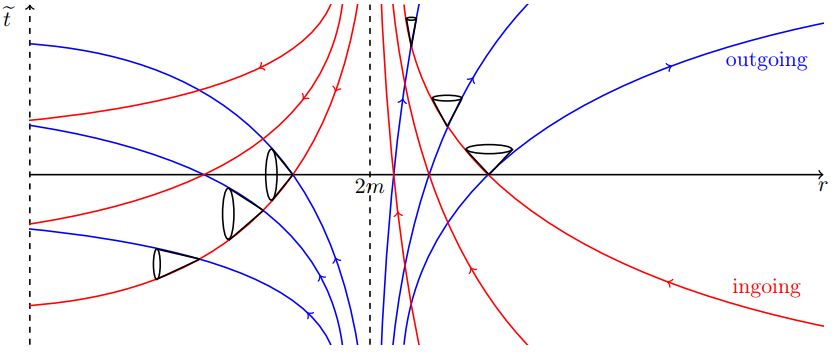
\includegraphics[width=0.9\textwidth]{Figuras/diag_schwc.png}
  \caption{diagrama de espaço-tempo em coordenadas de Schwartzchild - \textit{outgoing} e
          \textit{ingoing} representam raios de luz se afastando, e se aproximando, respectivamente. \\Fonte: Schuller, Dadhley (2015, p. 130)\cite{schuller2015}}
  \label{fig:diag_schwc}
\end{figure}

Note a distorção sofrida pelos cones de luz ao se aproximarem e se afastarem do horizonte de eventos. Note também que
esse diagrama, representado com essas coordenadas, poderia nos levar à conclusão de que as geodésicas tipo luz \textit{ingoing} (indo em direção ao buraco negro)
nunca atravessariam o horizonte de eventos, o que parece estar longe da verdade. Contudo, isso é o que nós observaríamos ao ver um objeto cair num
buraco negro de Schwartzchild, nunca veríamos esse objeto cruzar o horizonte de eventos - chegaria num ponto em que
ele aparecia \enquote{parado} em relação a nós, observadores, mas puramente devido a um fenômeno de dilatação
temporal extrema\footnote{como pode ser visto pelo lado esquerdo da equação (\ref{eq:dilat_temporal}) à medida que se toma $r \to 2GM^{+}$.}.  

Além de tudo isso, o diagrama $(t,r)$ nas coordenadas de Schwartzchild também pode nos levar a crer que a singularidade
$r=0$ é uma posição no espaço a ser alcançada, quando na verdade, veremos que se trata mais de uma \enquote{posição no tempo}\footnote{Tecnicamente, dizemos que a coordenada radial se torna tipo tempo, ou \textit{timelike}, que pode ser visualizada na figura \ref{fig:diag_schwc} pela \enquote{inversão} de direção dos cones de luz.},
a qual é impossível de ser evitada.

Em geral, alguns dos problemas encontrados em diagramas $(t,r)$ com coordenadas de Schwartzschild são resolvidos puramente por uma
escolha melhor de coordenadas, podendo ainda manter a forma cartesiana do diagrama. Contudo, propriedades mais fundamentais do espaço-tempo
na influência de buracos negros serão ainda mais elucidadas com os Diagramas de Carter-Penrose, como pretendemos mostrar nas próximas sessões deste trabalho.
\section{Transformações Conformes}

Um dos pilares dos diagramas de Carter-Penrose, e na verdade, onde reside o \textit{core}
da ideia principal desses diagramas, é justamente a noção de \textbf{Transformações Conformes}, juntamente com a de \textbf{compactação}, que trataremos mais adiante.

Até onde estamos interessados aqui para a construção desses diagramas, uma transformação conforme é 
basicamente uma mudança na geometria (portanto, uma mudança da métrica) que mantenha a estrutura causal do espaço-tempo
inalterada. Partiremos agora para a definição matemática, formal, e mais precisa do queremos dizer com isso.

\begin{definição}
(Transformação Conforme)\\\\
Uma \textit{transformação conforme} é uma mapa de um espaço tempo $(\mathcal{M},g)$
no espaço-tempo $(\mathcal{M},\tilde{g})$, dado por
\begin{equation*}
  \tilde{g}_{\mu\nu}(x) = \omega^2(x)g_{\mu\nu}(x)
\end{equation*}
com $\omega \in C^{\infty}(\mathcal{M})$, e tal que $\omega(x) \neq 0, \forall x \in \mathcal{M}$; onde $x$ representa o conjunto das coordenadas $x^{\mu}$ avaliado num certo ponto do espaço-tempo.
\begin{flushright}
  \qed
\end{flushright}
\end{definição}
Segue da condição $\omega^2(x)>0$, que curvas tipo tempo/luz/espaço sob a métrica $g_{\mu\nu}$ também o serão para a 
métrica conforme $\tilde{g}_{\mu\nu}$:
\begin{align*}
   \tilde{g}(u_{\gamma},u_{\gamma}) &< 0 \Longleftrightarrow  g(u_{\gamma},u_{\gamma}) < 0\\
   \tilde{g}(u_{\gamma},u_{\gamma}) &= 0 \Longleftrightarrow  g(u_{\gamma},u_{\gamma}) = 0\\
   \tilde{g}(u_{\gamma},u_{\gamma}) &> 0 \Longleftrightarrow  g(u_{\gamma},u_{\gamma}) > 0.
\end{align*}
Além disso, a segunda condição acima garante que geodésicas tipo luz sob uma métrica também o serão
para a outra métrica, o que não vale de modo geral para geodésicas tipo tempo/espaço sob $g$, pois elas não
são necessariamente mapeadas em \textit{geodésicas} sob $\tilde{g}$.

É com essas 3 últimas expressões que queremos dizer com \enquote{preservam a estrutura causal}.

\section{\enquote{Receita} para Diagramas de Penrose}
\section{Coordenadas de Krushal-Szekeres}
\section{Aplicações Simples do Diagrama de Penrose}
\section{Conclusão}





% --- BIBLIOGRAFIA ---
\newpage
\pagenumbering{gobble}
\nocite{*}
\printbibliography[title={Referências}]

\end{document}